% Updated in September 2014 by Hideo Saito
% Updated in September 2012 by In Kyu Park
% Updated in April 2002 by Antje Endemann, ...., and in September 2010 by Reinhard Klette
% Based on CVPR 07 and LNCS style, with modifications by DAF, AZ and elle 2008, AA 2010, ACCV 2010, ACCV 2012

\documentclass[runningheads]{llncs}
\usepackage{graphicx}
\usepackage{amsmath,amssymb} % define this before the line numbering.
\usepackage{color}
\usepackage{epstopdf}
\usepackage{epsfig}
\usepackage{bm}
\usepackage{url}
%===========================================================
\begin{document}

%macro for raising the point in decimal numbers; see example in the abstract
\newcommand{\point}{
    \raise0.7ex\hbox{.}
    }

%Do   -- NOT --    use any additional macros

\pagestyle{headings}

\mainmatter



%===========================================================
\title{Clouds in The Cloud} % Replace with your title

\titlerunning{Clouds in The Cloud} % Replace with your title

\authorrunning{Dmitry Veikherman, Amit Aides, Yoav Y. Schechner and Aviad Levis} % Replace with your names

\author{Dmitry Veikherman, Amit Aides, Yoav Y. Schechner and Aviad Levis} % Replace with your names
\institute{Dept. of Electrical Engineering, Technion - Israel Inst. of Technology, Haifa, Israel} % Replace with your institute's address
\maketitle

%===========================================================
\begin{abstract}
Light-field imaging can be scaled up to a very large area, to map the Earth's atmosphere in 3D. Multiview spaceborne instruments suffer low spatio-temporal-angular resolution, and are very expensive and unscalable. We develop sky light-field imaging, by a wide, scalable network of wide-angle cameras  looking upwards, which upload their data to the cloud. This new type of imaging-system poses {\em new computational vision and photography problems}, some of which generalize prior monocular tasks. These include radiometric self-calibration across a network, overcoming flare by a network, and background estimation. On the other hand, network redundancy offers {\em solutions} to these problems, which we derive. Based on such solutions, the light-field network enables unprecedented ways to measure nature. We demonstrate this experimentally by 3D recovery of clouds, in high spatio-temporal resolution. It is achieved by space carving of the volumetric distribution of semi-transparent clouds. This sensing approach can complement satellite imagery, be useful to aviation meteorology, make aerosol tomography realizable, and give new, powerful tools to atmospheric and avian wildlife scientists.

\end{abstract}

%===========================================================
\section{Introduction}

Plenoptic, light-field and integral imaging~\cite{Adelson1992,Basha2012,bishop,horstmeyer,Ng1948,kim,Stelamaris2014} sample the radiance distribution in location and direction. This imaging mode has been used mainly in small-scale setups. However, it can be scaled up to map the Earth's atmosphere in 3D. Sampling the atmospheric radiance spatio-angularly is achieved by a few spaceborne and airborne instruments, including the Multiangle Imaging SpectroRadiometer (MISR)~\cite{diner,Diner1998}, the Airborne Multiangle SpectroPolarimetric Imager (AirMSPI)~\cite{dinerDavis07,dinerDavis10} and POLDER~\cite{baxter,breon,vanMol}.
These architectures have crude resolution spatially (effectively several kilometers per pixel), angularly ($\approx 7$ angles per view)~\cite{5753124}, and temporally (orbit takes several days to return to the same terrestrial spot). Furthermore, spaceborne instruments are extremely expensive and unscalable. We develop a counter approach: the atmospheric light-field is captured  from below, by wide-angle cameras looking upwards. Contrary to super-expensive one-off instruments, our approach is a {\em scalable sensor network}, that captures images simultaneously over a very large area, densely.

Creating and exploiting such a network poses several requirements: low-cost units,
communications, and tailored computational photography algorithms. The first two requirements are met  thanks to wireless infrastructure, low-cost cameras and {\em cloud computing} services. Hence, we can deploy solar-powered cameras at will, nearly anywhere. By wireless, they upload their sky-images to the ``cloud'', from which the light-field data can be analyzed. However, this new type of imaging-system gives rise to new problems and algorithms, part of which we deal with in this paper. In a sense, the network generalizes some problems that had been posed for monocular setups a decade ago. On the other hand, network redundancy offers {\em solutions} to these problems.

The computational photography problems include radiometric self-calibration across a network of cameras, background estimation, and overcoming saturation and flare by a network. We demonstrate this in real field experiments by building a small version Sky-Technion Array of Sensors (STARS). The network enables unprecedented 3D imaging of clouds, in high spatio-temporal resolution. This approach can complement multi-angular satellite imagery. It can make aerosol tomography~\cite{Aides:13,Tomography2014} realizable, offer new ways to study weather phenomena and avian wildlife, and aid electric power management~\cite{Peng2014}.



%%%%%%%%%%%%%%%%%%%%%%%%%%%%%%%%%%%%%%%%%%%%%%%%%%%%%%%%%%%%%%
\section{Background}
\label{sec:theory}


%%%%%%%%%%%%%%%%%%%%%%%%%%%%%%%%%%%%%%%%%%%%%%%%%%%%%%%%%%%%%%
\subsection{Monocular radiometric self-calibration}
\label{sec:Signelradio}

A large network should use low-cost camera units. Such cameras often have spatial and temporal radiometric inconsistencies. For example, spatial gain (e.g., by vignetting~\cite{LitvinovCVPR05,Kang2000}) is often modeled by a function $M({\bf x})$, where \mbox{${\bf x}=(x,y)$} is a camera pixel. The image pixel irradiance at time $t$ is
\mbox{$ \tilde{I}_t({\bf x}) = M({\bf x})I_t(O)$}, where $I_t(O)$ is the pixel irradiance when $M=1$, for observed object $O$. For a single camera, consistent readouts can be obtained in the field by self-calibration. The strongest methods rely on redundant images, taken at modulated settings.
Correspondence is established between modulated measurements, e.g. by aligning a pan sequence. Assuming brightness constancy, corresponding measurements yield constraints.

%\begin{equation}
% \log M({\bf x})- \log M({\bf x}')=\log \tilde{I}_t({\bf x})-\log \tilde{I}_t'({\bf x}').
% \label{eq:logM}
%\end{equation}
Aggregating constraints over different pixels and frames recovers parameters of radiometric inconsistencies. This recovery makes monocular pixel readout spatially consistent. In Sec.~\ref{sec:mutiradio} we expand this principle to a camera-array.



%%%%%%%%%%%%%%%%%%%%%%%%%%%%%%%%%%%%%%%%%%%%%%%%%%%%%%%%%%%%%%
\subsection{Avoiding Blooming, Lens-Flare in a Single Camera}
\label{sec:Signelflare}

In wide-angle sky-views, sun-rays are liable to frequently shine directly into the lens, creating blooming. Moreover, sun-rays create an additive, spatially varying lens-flare. Reducing flare was suggested~\cite{Koreban2009,Raskar2008,Talvala2007,Rouf2011} using either a specialized detector array for nearby objects, or camera rotation during capture of a static scene. Both approaches complicate the need for simple, low-cost units and operation.
%Third, direct sunlight repeatedly entering the camera chamber and hitting pixels may damage the camera after a while.

Sky-observing wide-field cameras often have a {\em dynamic sun blocker}: an opaque object raised above the camera optics, blocking the Sun from view. There are various configurations, but all of them {\em move}, as the Sun direction changes during the day and across the year. Motorized solutions~\cite{Pust2008} that need to work year-around significantly complicate such camera units, making them very expensive. Sec.~\ref{sec:mutiSun} explains that a large camera network inherently bypasses the problem, without a need to constantly move a Sun blocker.




%%%%%%%%%%%%%%%%%%%%%%%%%%%%%%%%%%%%%%%%%%%%%%%%%%%%%%%%%%%%%%
\subsection{Current 3D Cloud Mapping}
\label{sec:current3D}

Existing sky-imaging systems used for research and operational meterology\footnote{There are also ground viewing webcams that happen to see sky parts~\cite{bradley,jacobs14cloudmap} and weather cameras
that are too sparse to be integrated for recovery.} are few, relying on high quality components~\cite{allmen,angeo-27-953-2009,cazorla,long,Seiz,kassianov}. Due to their complexity and costs, they were only used to estimate {\em cloud-base} over narrow regions right above a narrow-baseline camera pair. Satellite-based estimation of 3D {\em cloud-tops} has been proposed by MISR~\cite{Seiz2006}. It takes several minutes for MISR to capture multiple viewpoints of a region, during which the clouds generally move. Weather radars sense {\em raindrops}, which are much larger than cloud-drops and ice crystals.

%%%%%%%%%%%%%%%%%%%%%%%%%%%%%%%%%%%%%%%%%%%%%%%%%%%%%%%%%%%%%%
\section{Regional Stationarity in a Camera Network}
\label{sec:station}

A network of sky-observing cameras is spread over a region. The location vector of camera $c$ is ${\bf l}_c$. Any image pixel ${\bf x}$ of camera $c$ is back-projected to a ray at direction-angle vector (zenith, azimuth) ${\bm \theta}$ in a global coordinate system. The data is the radiance measured per location, direction and time, $\tilde I_t[{\bf l}_c,{\bm \theta}(\bf x)]$.
An interesting assumption that can be made is {\em regional stationarity}. In a region containing the cameras, the chance of a cloud, clear sky, or haziness affecting $\tilde I_t[{\bf l}_c,{\bm \theta}]$ is {\em independent} of $c$. Thus, inter-camera image variations due to atmospheric conditions are {\em random and unbiased}. This is illustrated in Fig.~\ref{fig:station}.
\begin{figure}[t!]
  \begin{center}
    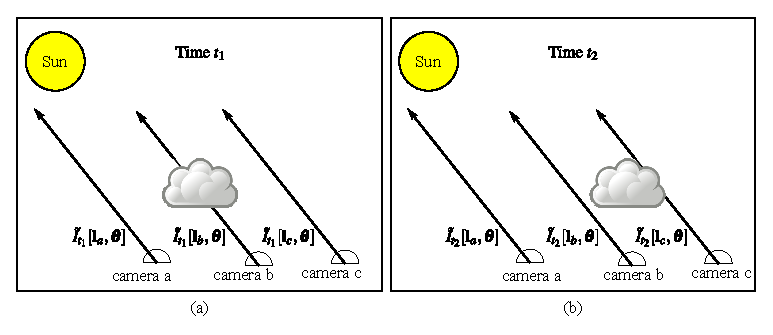
\includegraphics[width=\linewidth]{regional_stationarity.eps}
  \end{center}
  \vspace{-0.6cm}
  \caption{  %[a] and [b] show the network at times $t_1$ and $t_2$ respectively.
    Regional stationarity: in a wide
    region, objects at infinity and the background
    sky should have the same color, for a common viewing angle ${\bm
      \theta}$, e.g.,
%    $\tilde I_{t_1}[{\bf l}_a,{\bm \theta}]$ vs. $I_{t_1}[{\bf l}_c,{\bm \theta}]$.
    $[{\bf l}_a,{\bm \theta}]$ vs. $[{\bf l}_c,{\bm \theta}]$ at $t_1$.
    Nearby objects (clouds) result in pixel differences, e.g.,
    $[{\bf l}_b,{\bm \theta}]$ vs. $[{\bf l}_c,{\bm \theta}]$ at $t_1$.
    Nevertheless, the light-field statistics (spatio-temporal variations and correlations) are stationary across viewpoints. This enables statistical processing  across viewpoints and time.  Residual measured bias is
    attributed to slight inter-camera radiometric inconsistencies.  }
  \label{fig:station}
\end{figure}

Some monocular algorithms tend to rely on gathering statistics over time, thus assuming temporal stationarity. Nevertheless, {\em simultaneous} images captured by {\em different camera nodes} are generally different from each other. Due to regional stationarity, a change of viewpoint has an effect similar to change in time: a cloud in
$\tilde I_t[{\bf l}_c,{\bm \theta}]$ is often not in $\tilde I_t[{\bf l}_{c'},{\bm \theta}]$. Consequently, monocular algorithms can be extended to statistics gathered over both time and viewpoint (as done underwater in~\cite{6528314}).
Regional stationarity is supported by meteorological research~\cite{lensky2006time,Mesoscale}.
Stationarity breaks down across large topographic discontinuities: a mountain ridge, coast line. These locations are known, and hence can be handled or avoided in stationarity-based analysis.



%%%%%%%%%%%%%%%%%%%%%%%%%%%%%%%%%%%%%%%%%%%%%%%%%%%%%%%%%%%%%%
\section{Self-Calibration in a Camera Network}
\label{sec:muticalib}

Before a camera is deployed in the field, its internal geometric and radiometric characteristics (including distortions, radiometric response) are calibrated in the lab. This is done using established monocular methods. However, once a camera is placed in the field, unknown parameters are introduced. External sources in the vicinity of a camera may create a weak lens glare, that {\em offsets} radiometric readings, in way that varies both spatially and across viewpoints. Moreover, residual {\em gain} variations may be between different cameras, despite lab calibration. This may be exacerbated in the field by dirt accumulation on lenses. Similarly to Sec.~\ref{sec:Signelradio}, the solution relies on redundant measurements at corresponding points.

For correspondence, geometric calibration~\cite{Seiz2002} is necessary. The internal parameters $\Psi_c$ of camera $c$ are pre-calibrated in the lab.
In the field, the location vector ${\bf l}_c$ is known by GPS but the orientation (yaw, pitch and roll angle vector ${\bf \Theta}_c$) is loosely set. The orientation is calibrated by automatically detecting and tracking extra-terrestrial (XT) objects (Moon, planets, Sun)~\cite{Seiz2002,lalonde}, across night or day\footnote{In~\cite{Seiz2002}, calibration relied on manual tracking of a special flight and long exposures at night.}, at pixel ${\bf x}^{\rm XT}_{\rm measured}(t)$. Using astronomical charts, an XT object is known\footnote{Atmospheric refraction is negligible: higher than 20$^{\circ}$ above the horizon, the refraction-error is less than 0.05$^{\circ}$~\cite{NAV:6418444}, much less than the angular size of each of our pixels, 0.18$^{\circ}$.} to be at angle vector (zenith, azimuth) ${\bm \theta}^{\rm XT}(t)$ relative to a global coordinate system. Given camera orientation ${\bf \Theta}_c$, a projection ${\Pi}$ converts a ray direction ${\bm \theta}^{\rm XT}(t)$ to pixel ${{\Pi}({\bm \theta}^{\rm XT}(t);{\bf \Theta}_c,\Psi_c)}$.

During the course of a day or night, the number of frames
  $N^{\rm frames}$ is ${\cal O}(100)$, leading to a simple optimization formulation:
\begin{equation}
 \hat{\bf \Theta}_c=\arg\min_{{\bf \Theta}_c}
 \sum_{t=1}^{N^{\rm frames}}
 \|{\Pi}({\bm \theta}^{\rm XT}(t);{\bf \Theta}_c,\Psi_c) - {\bf x}^{\rm XT}_{\rm measured}(t)\|^2
\;.
 \label{eq:hatThetac}
\end{equation}
We solved it using exhaustive search or gradient descent from null initialization, with the same results. The orientation calibration is illustrated in Fig.~\ref{fig:sunmotion}.


\begin{figure}[t!]
\begin{center}
   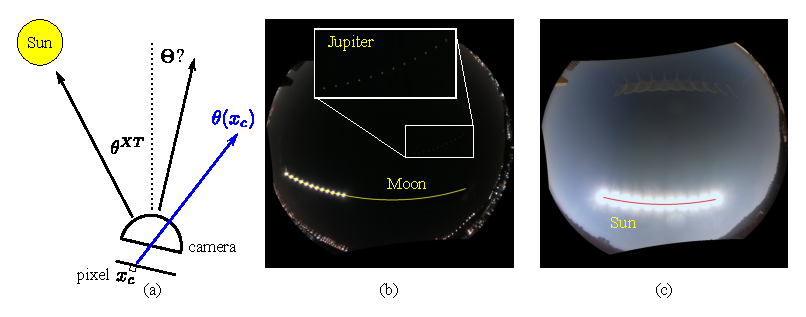
\includegraphics[width=0.9\linewidth]{sun_moon.eps}
\end{center}
   \vspace{-0.6cm}
   \caption{(a) To estimate the camera yaw-pitch-roll angle vector ${\bf \Theta}_c$, we rely on
   image locations of extra-terrestrial objects, whose direction vector ${\bm \theta}^{\rm XT}(t)$
   is known $\forall t$. (b) Photo-montage of night sky images. It shows the Moon at different times, the expected trajectory based on the estimated ${\bf \Theta}_c$, and a close-up on the corresponding sampled images of Jupiter. (c) Photo-montage of the daylight sky. It shows the Sun at different hours, the expected trajectory based on the estimated ${\bf \Theta}_c$ and lens-flares.
   }
\label{fig:sunmotion}
\end{figure}
Based on $\hat{\bf \Theta}_c$, all captured images $\tilde I_{c,t}(\bf x)$ taken by camera $c$ are aligned to the global coordinate system:
%Any image pixel ${\bf x}$ of camera $c$ is
the backprojected ray has direction vector %${\bm \theta}({\bf x})$ is given by
\begin{equation}
 {\bm \theta}({\bf x})={\Pi}^{-1}({\bf x};\hat{\bf{\Theta}}_c,\Psi_c)
  \;.
 \label{eq:thetac}
\end{equation}
%The sampled light-field is the radiance measured per location, direction and time, thus given by
%$\tilde I_t[{\bf l}_c,{\bm \theta}(\bf x)]$.



%%%%%%%%%%%%%%%%%%%%%%%%%%%%%%%%%%%%%%%%%%%%%%%%%%%%%%%%%%%%%%
\subsection*{Inter-camera Relative Radiometric Self-Calibration}
\label{sec:mutiradio}

%
%%%%%%%%%%%%%%%%%%%%%%%%%%%%%%%%%%%%%%%%%%%%%%%%%%%%%%%%%%%%%%%
%\subsection*{The Experimental Setup}
%\label{sec:system}
%

Consider a {\em fixed} view direction ${\bm \theta}$ observed by several cameras.
%, e.g., $c$ and $c'$.
The set $\{\tilde I_t[{\bf l}_c,{\bm \theta}]\}_c$ corresponds to readouts of parallel rays, back-projected from all cameras in the network. Values in this set generally differ from each other:
 $\tilde I_t[{\bf l}_c,{\bm \theta}]\neq \tilde I_t[{\bf l}_{c'},{\bm \theta}]$. There are two causes for this difference:\\
 {\tt 1}.~ Different camera locations mean different observed objects. Momentarily, camera $c$ may observe a cloud while $c'$ observes a clear sky, or vice versa. Camera $c'$ may momentarily observe a somewhat denser haze volume than $c$, etc. \\
 {\tt 2}.~ Slight inter-camera radiometric inconsistencies, which we need to estimate.\\
 \vspace{-0.2cm}

Cause {\tt 1} is usually dominant. We need to overcome it, in order to analyze cause {\tt 2}. Here we rely on the regional stationarity described in Sec.~\ref{sec:station}.
Per camera $c$ and view angle ${\bm \theta}$, bias is due to cause ({\tt 2}). We easily detect and characterize the bias by capturing {\em statistics over time}.


We performed experiments, with a small field-deployed network (STARS), detailed in Sec.~\ref{sec:set}. Figure~3a shows radiometric inconsistency between cameras $a$ and $b$. Figure~3b then shows a scatter-plot of
$\tilde I_t[{\bf l}_a,{\bm \theta}]$ vs.~$\tilde I_t[{\bf l}_{b},{\bm \theta}]$, $\forall t,{\bm \theta}$, for the red-channel.
\begin{figure}[t!]
\begin{center}
   \includegraphics[width=\linewidth]{bias4.eps}
\end{center}
   \vspace{-0.6cm}
   \caption{[a] Splitting the field of view to upper/lower halves, to pixels corresponding
   respectively to either $\tilde I_t[{\bf l}_a,{\bm \theta}]$  or $\tilde I_t[{\bf l}_{b},{\bm \theta}]$. In the line between the marked arrows, radiometric inconsistency shows-up as a seam across which colors slightly change ({\bf please view on a color computer screen}). [b] Scatter-plot of
   $\tilde I_t[{\bf l}_a,{\bm \theta}]$ vs.~$\tilde I_t[{\bf l}_{b},{\bm \theta}]$, $~\forall t,{\bm \theta}$, red-channel. [c] The estimated offset map ${\hat o}_{b-a}({\bm \theta})$, red channel. It is derived based on a set of images taken during several hours.
   [d]~Splitting the field of view in half, to {\em corrected} pixels from either
   $\hat I_t[{\bf l}_a,{\bm \theta}]$  or $\hat I_t[{\bf l}_{b},{\bm \theta}]$: inconsistencies in the line between the marked arrows are greatly
   diminished.
   }
\label{fig:calibration}
\end{figure}
From such plots, we hypothesized that camera $a$ has a slight offset, particularly in the red channel, relative to camera $b$. We thus estimated, per color channel, the map of radiometric offset (across pixels, or ray-directions). A temporal median was used:
\begin{equation}
 {\hat o}_{b-a}({\bm \theta})=
  {\rm median}_{t} \{\tilde I_t[{\bf l}_b,{\bm \theta}]-\tilde I_t[{\bf l}_a,{\bm \theta}]\}.
 \label{eq:hato}
\end{equation}
The map ${\hat o}_{b-a}({\bm \theta})$ was then spatially smoothed and used to correct $\tilde I_t[{\bf l}_a,{\bm \theta}]$. As shown in Fig.~\ref{fig:calibration}d, the results have much better inter-camera consistency. A similar process was applied to other cameras, but they had negligible radiometric offsets with respect to camera $b$. The spatially varying offset in camera $a$ was later found to be due to a nearby light source.

The process was then repeated to detect slight local variations of gain (vignetting). Suppose there is no offset. In analogy to Eq.~(\ref{eq:hato}), the gain in $b$ is higher than in $a$ by a factor
\begin{equation}
 {\hat M}_{b/a}({\bm \theta})=
  {\rm median}_{t} \{\tilde I_t[{\bf l}_b,{\bm \theta}]/\tilde I_t[{\bf l}_a,{\bm \theta}]\}.
 \label{eq:hatm}
\end{equation}
This way, all the network is radiometrically aligned to a single master camera.
After radiometric corrections, the light-field samples are denoted $\hat I_t[{\bf l}_b,{\bm \theta}]$.


 %%%%%%%%%%%%%%%%%%%%%%%%%%%%%%%%%%%%%%%%%%%%%%%%%%%%%%%%%%%%%%
\section{More Details About The Experimental Setup}
\label{sec:set}

Before proceeding with mathematical problems and solutions, we give more details about a small version STARS network, which we built. Each of the five camera nodes (units) was built from basic components, and coarse alignment tolerances. Its core is a Raspberry-Pi computer and a 5MP Raspberry-Pi camera. In this camera, the gain, response and white-balance can be fixed, avoiding temporal radiometric variations. We manually mounted a small fisheye lenses. Due to this coarse lens-to-chip alignment, each camera has a different peripheral dead-region, creating a missing part in the hemispheric view-field and vignetting distinct to each camera (Fig.~\ref{fig:photomotion}). As we explain, a {\em {\em network} as-a-whole} can inherently overcome these issues. Every 30 seconds, synchronously, all units automatically transmit image data to the internet (cloud-service). Each unit is solar powered.
STARS used several rooftops at the Technion and ran for weeks, capturing 70GB of sky imagery~\cite{download}.
\begin{figure}[t!]
\begin{center}
   \includegraphics[width=1\linewidth]{scene_d.eps}
\end{center}
   \vspace{-1.2cm}
   \caption{Images taken simultaneously by a 5-node STARS network. They are geometrically aligned to the zenith and north, and resampled to {\em polar azimuthal equidistant} projection in this global system. Equidistant zenith angle circles are overlayed on $\tilde I_t[{\bf l}_e,{\bm \theta}]$ (camera $e$). Each camera had dead-regions, due to rough lens alignment.
   Corresponding to the frame in camera $e$, a {\em cloud score} map (Eq.~\ref{eq:sr}) has high values in cloud-pixels, diminishing outside them. [Bottom-right] The 3D setup of STARS, laterally spread over hundreds of meters, at somewhat different altitudes.}
\label{fig:photomotion}
\end{figure}


%%%%%%%%%%%%%%%%%%%%%%%%%%%%%%%%%%%%%%%%%%%%%%%%%%%%%%%%%%%%%%
\section{Network-assisted Background Estimation}
\label{sec:background}

In monocular settings, change-detection algorithms use temporal filtering to characterize the background: foreground dynamic objects are at {\em different locations at different times} and are thus pruned. In our case this translates to stating that a cloud in
$\tilde I_t[{\bf l}_c,{\bm \theta}]$ is often not in
$\tilde I_{t'}[{\bf l}_c,{\bm \theta}]$, when $t'\neq t$. However, if clouds move slowly, while illumination gradually changes, temporal filtering may be insufficient. This is illustrated in Fig.~\ref{fig:sky}.

A light-field network enhances this principle, with more effective pruning-per-time.
Recall regional stationarity (Sec.~\ref{sec:station}). A change of viewpoint has an effect similar to change in time: a cloud in
$\tilde I_t[{\bf l}_c,{\bm \theta}]$ is often not in $\tilde I_t[{\bf l}_{c'},{\bm \theta}]$. Consequently, background sky values are obtained by data filtering over {\em both} time and viewpoint.

This network-based principle can enhance existing or future algorithms of background estimation, which would otherwise be monocular. A demonstration, shows results using a simplistic, basic criterion. In broad daylight, clouds are brighter than the sky~\cite{hosek2012analytic}. Hence, an estimator for the sky background can be, for example
\begin{equation}
 {\rm SKY}({\bm \theta})= \arg\min_{t,c} \tilde I_t[{\bf l}_c,{\bm \theta}]
 \label{eq:SKY}
\end{equation}
where $t\in[1\ldots N^{\rm frames}]$ and $c\in[1\ldots N^{\rm views}]$.
This is illustrated in Fig.~\ref{fig:sky}.
\begin{figure}[t!]
\begin{center}
   \includegraphics{Background.eps}
\end{center}
   \vspace{-0.6cm}
   \caption{[Left] Estimation of the sky background, using Eq.~(\ref{eq:SKY}) based on five temporal instances and five viewpoints. [Right] Estimation of the sky background, using five temporal instances, but just a single viewpoint, resulting in more residual clouds.}
\label{fig:sky}
\end{figure}


%%%%%%%%%%%%%%%%%%%%%%%%%%%%%%%%%%%%%%%%%%%%%%%%%%%%%%%%%%%%%%
\section{Bypassing the Sun Through a Camera Network}
\label{sec:mutiSun}

As Sec.~\ref{sec:Signelflare} explains, in existing full sky-imagers, effects of direct sunlight are often mitigated by a small dynamic sun-blocker, which complicates the system and its cost, while having a blind-region. The network offers a different solution, which can be radical, yet simple. On each camera, the sun-blocker is {\em static}, and has no moving part. The blocker can be large, covering the entire range of directions the Sun may occupy during the year or part of it. In this configuration, each camera unit has a large blind area (See Fig.~\ref{fig:blindspot}). Nevertheless, the entire {\em network has no blind spot}, when viewing the atmosphere. This remarkable property is a result of network-redundancy, as we explain.
\begin{figure}[t!]
\begin{center}
   \includegraphics[width=0.99\linewidth]{sun_blocks2.pdf}
\end{center}
   \vspace{-0.6cm}
   \caption{[a] Camera $c$ has a blind-region, covering Sun directions at ${\bf l}_c$. The blind region corresponds to set $\Gamma_c$ of atmospheric voxels not sensed by by camera $c$. The network as a whole still has coverage of voxels $k\in\Gamma_c$, as they are observed by cameras $e,f,g$.
   [b] Simulation of a whole sky image (polar azimuthal equidistant projection), blocking
   all solar directions during the year, at a mid-latitude.
   [c] In the topics, the network must have nodes at distance $D$ outside surveyed area ${\cal A}$, if ${\cal A}$ is narrow.  The distance D depends on the latitude $\gamma$, while
   $\beta\approx23.5^o$.
   [d] In the arctic, the blind region is adjacent to the horizon, in all azimuth angles. Fixed blocking of the Sun over $360^o$  blocks low-altitude voxel $k$. [e] Arctic cameras fitted with a fixed north-facing sun blocker create a network   that operates 12 hours a day. An adjacent camera at each node has a fixed south-facing sun blocker, for imaging during complementing hours.
   %For tropic cameras, the blind region dissects the field from east to west through the Zenith. In the arctic, the blind region is adjacent to the horizon.
   }
\label{fig:blindspot}
\end{figure}


A static year-round sun blocker on camera $c$ permanently obstructs a set $\Gamma_c$ of atmospheric voxels. These voxels, however, are generally visible at several other cameras, e.g., those indexed $e,f,g$ in Fig.~\ref{fig:blindspot}. Consequently, a sufficiently wide network has no 3D blind spot, despite permanent sun-blocking. Voxels that are not obstructed from any camera have more viewpoints to constrain their content, than voxels in $\Gamma_c$.

We now quantify the implication of this approach to the network extent, referring to the northern hemisphere without loss of generality.
Nearly all weather phenomena are under the tropopause, whose altitude $H$ above sea level is typically 17km at the equator, and decreasing with latitude. The solar seasonal angle amplitude is $\beta\approx23.5^o$. At latitude $\gamma$, thus, a permanent sun blocker spans zenith angles in the range $\gamma\pm\beta$. Earth is divided here to three region classes:\\
  ${\bf \bullet}$ In the tropics, the sky directly above a camera is blocked. Consider
  a small tropical area ${\cal A}$, e.g., 1km wide, whose sky needs to be monitored. According to Fig.~\ref{fig:blindspot}c, ${\cal A}$ can efficiently be observed without
  a blind spot by cameras to its {\em south}. The network needs to have camera units extending to distance  $D=H\tan(\beta-\gamma)+\epsilon$ from ${\cal A}$, where $\epsilon$ is a small distance, sufficient for triangulation at $H$. At the equator $D\approx7.4$km.
  It can also be shown that if ${\cal A}$ is wider than $2H[\tan(\beta-\gamma)+\tan(\beta+\gamma)]$, the network can observe and triangulate all the sky right above it.\\
${\bf \bullet}$  As latitude increases towards the tropic circles, $D$ decreases to zero. Thus the network can observe and triangulate all the sky right above it, anywhere outside the tropics, in the mid-latitudes.\\
  ${\bf \bullet}$ In the arctic and antarctic summer, the Sun can appear in all azimuth angles over the day. A single 24-hour fixed sun-blocker blocks the horizon. So as shown in Fig.~\ref{fig:blindspot}d, voxel $k$ is not observed. One solution would be to mount two cameras, side by side, in each network node. Each camera in a node has a fixed sun blocker, covering half of the azimuth angles. One camera operates in the {\em polar daytime} (local 6AM to 6PM), as it has a south-oriented fixed blocker. The other camera operates in the complementing time (Fig.~\ref{fig:blindspot}e), having a north-oriented fixed blocker. This way, the network never has a blind spot.


%%%%%%%%%%%%%%%%%%%%%%%%%%%%%%%%%%%%%%%%%%%%%%%%%%%%%%%%%%%%%%
\section{3D Clouds by a Camera Network}
\label{sec:3Dc}

One application is estimation of the 3D cloud field above the network domain, and beyond. This can be done by the following steps:~ 
({\tt A})~Per time $t$, give a {\rm cloud score} $s$  to each ray $[{\bf l}_c,{\bm \theta}]$, as we explain below.~({\tt B})~Perform a fuzzy version of space carving~\cite{Kutulakos2000,Ihrke2004}.

We first describe a simple method to implement ({\tt B}).  The set of all sampled light-field rays is ${\cal R}$, where
\mbox{$|{\cal R}|=N^{\rm rays}$}. A ray is indexed by $r$, and it corresponds to a specific $[{\bf l}_c,{\bm \theta}]$. Voxel $k$ projects to a subset of the rays $\rho_k\subset{\cal R}$,
that reach $\nu_k$ viewpoints. Suppose a ray $r\in{\cal R}$ has a cloud-score $s(r)\in[0,1]$, where \mbox{$s=0$} means there is definitely no cloud on the ray, while \mbox{$s=1$} means there is confidently a cloud there. Per voxel $k$, define a back-projected score
\begin{equation}
 B_k= \left[ \prod_{r\in\rho_k} s(r)\right]^{1/|\rho_k|}
 \;\; ~~{\rm if}~~ \nu_k\geq 2
  \;.
 \label{eq:Bk}
\end{equation}
The back-projected score of voxel $k$ is null, if $k$ is not observed by at least two viewpoints. This score is null also if $s(r)=0$ for any $r\in\rho_k$. If all $r\in\rho_k$ have same score $s$, then $B_k=s$. Equation~(\ref{eq:Bk}) carves-out voxels that contradict support for clouds.

Different cloud regions have signature appearances. Ignoring this would allow erroneous matching of, say, a darker cloud-bottom to a bright sun-lit side of a cloud, or a smooth cloud region to a textured one. Thus, photometric and appearance consistency across viewpoints is incorporated (the photo-hull concept in space-carving~\cite{Kutulakos2000}).
From the images, a feature vector ${\bf v}(r,t)$ is extracted for any measured ray $r$.
We used SIFT descriptors~\cite{lowe2004distinctive} and the radiance in each color channel. Element $q$ of ${\bf v}(r,t)$ is $v_q(r,t)$. The values of this element, for all rays that intersect voxel $k$, is \mbox{${\cal V}_q(k,t)\equiv\{v_q(r,t)\}_{r\in\rho_k}$}.
Across viewpoints, the measured variance in this set is
${\rm VAR}[{\cal V}_q(k,t)]$. Define an appearance consistency score~\cite{Supp2014} as
\begin{equation}
 P_k= \exp\left(
         -\Sigma_q\{{\rm VAR}[{\cal V}_q(k,t)]\}/\sigma^2
         \right)
  \;,
 \label{eq:Dist}
\end{equation}
where $\sigma^2$ is a scale parameter. The total cloud-score of a voxel is \mbox{$T_k=B_kP_k$}.
The resulting 3D field $\{T_k\}$ is a volumetric estimate of cloud occupancy. It is biased to yield clouds larger than they really are: high-altitude voxels occluded by the cloud-base from all viewpoints are interpreted as being cloudy, since for them $T_k$ is high. This is a realization of a basic ambiguity: if a voxel is occluded from all viewpoints, then there is no way of telling if it is cloudy or not, unless auxiliary or prior knowledge is available. Incorporating a visibility prior favors smaller clouds that explain the data. If voxel $k$ is completely occluded by other cloudy voxels, then it can be pruned (carved) out. Voxel $k$ can maintain its $T_k$ if there are at least two camera viewpoints from which $k$ is not occluded by other clouded voxels. Pruning is achieved by sweeping~\cite{Kutulakos2000} the field $\{T_k\}$ iteratively. The pruned 3D cloud occupancy field is denoted $\{\tilde T_k\}$. We can maintain the non-binary (fuzzy) nature or $\{\tilde T_k\}$. This way, it possesses the inherent semi-transparency and subtle ambiguity of clouds.

%%%%%%%%%%%%%%%%%%%%%%%%%%%%%%%%%%%%%%%%%%%%%%%%%%%%%%%%%%%%%%
\subsection*{Basic cloud score}
\label{sec:cloudscore}


In the literature there are various functions for a basic cloud score (step {\tt A}). There is room for increased sophistication, including machine learning~\cite{Peng2014}. However, a ratio of image readout at the red/blue color channels, $\tilde I^{\rm red}/\tilde I^{\rm blue}$, is widely used~\cite{Seiz2002,Yamashita2004}. Overall, we found it effective in broad daylight: clouds are grey (unit red-blue ratio), and the cloudless sky is significantly biased to blue
(below $\approx 0.8$ red-blue ratio). Thus, for demonstrations in this paper,
the cloud-score we used per ray (pixel) is
\begin{equation}
 s(r)=\left\{
      \begin{array}{ll}
      \frac{6 [\tilde I^{\rm red}(r)/\tilde I^{\rm blue}(r)-0.8]}
           {0.2+\tilde I^{\rm red}(r)/\tilde I^{\rm blue}(r)}
      & ~~~~{\rm if}~ \tilde I^{\rm red}(r)/\tilde I^{\rm blue}(r)>0.8 \\
      0
      & ~~~~{\rm otherwise}
      \end{array}
      \right.
  \;.
 \label{eq:sr}
\end{equation}
Here $s\in[0,1]$, where either bound is achieved at gray clouds or blue sky, respectively. An example of applying this operator on an image is shown in Fig.~\ref{fig:photomotion}.



%%%%%%%%%%%%%%%%%%%%%%%%%%%%%%%%%%%%%%%%%%%%%%%%%%%%%%%%%%%%%%
\subsection*{Simulations}
\label{sec:simulation}

Quantitative assessments used atmospheric-science simulators.
An atmosphere over $8\times8{\rm km}$  was produced using off-the-shelf large eddy simulation (LES), creating clouds between heights of $500{\rm m}$ to $1500{\rm m}$.
Lighting conditions were consistent with Copenhagen.
Radiative transfer using the discrete ordinate spherical-harmonic method (SHDOM)~\cite{Evans1998} rendered images taken by 100 cameras in a $2.5\times 2.5{\rm km}^2$ domain. Recovery simulations used random subsets
of the network, where the whole network is either with or without
a sun blocker. In the LES, a voxel is occupied by cloud if its water-mass parameter is not null. In the recovery, voxel $k$ is classified as cloud if $T_k>0.01$.
We measured the classification error rate, across all voxels.
The results are plotted in Fig.~\ref{fig:simulations}. 
\begin{figure}[t]
  \begin{center}
    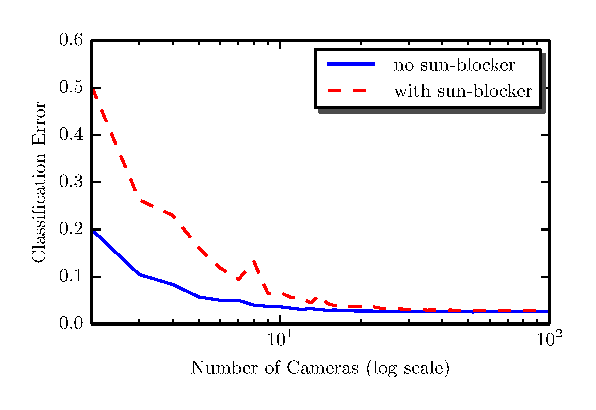
\includegraphics[width=0.65\linewidth]{simulations.eps}
    \vspace{-0.2cm}
    \caption{Classification error rate vs.~{$N^{\rm views}$}. Without or with a sun blocker.  Fluctuations are within the random sampling standard deviation.}
    \label{fig:simulations}
  \end{center}
\end{figure}
\begin{figure}[h!]
\begin{center}
   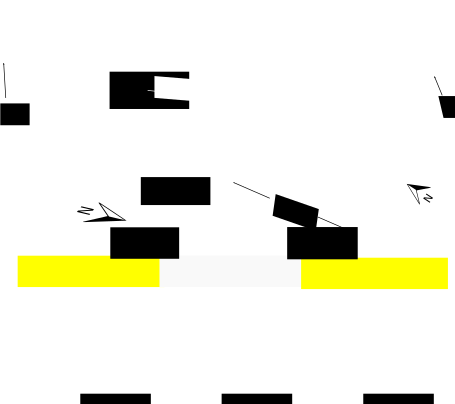
\includegraphics[width=0.95\linewidth]{clouds_reconstructions.pdf}
\end{center}
   \vspace{-0.6cm}
   \caption{3D cumulus cloud recovery results. (a,b) Cross-sections of the recovered cloud-occupancy field $\{\tilde T_k\}$. The domain of the clouds is much larger than STARS. Cloud
   altitude is above sea-level. (c) Estimated sky-background image.  Based on four viewpoints (indexed $a,b,c,d$), the 3D volumetric cloud-occupancy field $\{\tilde T_k\}$ was derived. The field $\{\tilde T_k\}$ was projected to viewpoint $e$, and overlayed on the estimated sky-background image. The resulting synthetic cloud-score image $J[{\bf l}_e,{\bm \theta}]$ is shown in (d). This can be compared to the real captured image $\hat I_t[{\bf l}_e,{\bm \theta}]$, shown in (e).}
\label{fig:projection}
\end{figure}
As expected of space carving,
results improve fast from 2 to 10 cameras. Even with a sun blocker,
the algorithm is able to reconstruct the cloud formation, but, more cameras are needed in order to compensate for the limited view of
each camera.


%%%%%%%%%%%%%%%%%%%%%%%%%%%%%%%%%%%%%%%%%%%%%%%%%%%%%%%%%%%%%%
\subsection*{Cloud Reconstruction Experiment}
\label{sec:results}

We applied the approach on various captured scenes.\footnote{Sun blocker was not used here, since saturation and blooming do not impair cloud shape reconstruction.} One scene had cumulus clouds, similar to those seen in Fig.~\ref{fig:photomotion}.
Cross-sections of the recovered 3D cloud-occupancy field $\{\tilde T_k\}$ are shown in Fig.~\ref{fig:projection}. The lateral domain of the clouds is much larger than STARS.
Accounting for the altitude of STARS above sea-level, the clouds mainly reside between 800m to 1450m above Sea-level. We used two indicators to validate the results. First, a balloon-based radiosonde measured the vertical humidity profile in Beit-Dagan, Israel. It is on a similar coastal strip, and roughly used by forecasters for our Technion location. It indicated a layer of high humidity that can yield clouds in the range $[770,1881]$m above sea-level, consistent with our clouds.

Second, we cross-validated 3D recovery {\em with a missing field of view}. We used four cameras (indexed $a,b,c,d$) out of five, for 3D estimation. Camera $e$ was ignored. Then, we projected the estimated 3D cloud distribution into viewpoint $e$, and compared to the ground truth. The rendered image is as follows. {\em Ray casting}~\cite{Levoy1990} of  field $\{\tilde T_k\}$ is performed on a ray corresponding to
$[{\bf l}_e,{\bm \theta}]$. Ray-casting aggregates $\{\tilde T_k\}$ on all voxels intersected by the ray. The result is a cloud-score image $w[{\bf l}_e,{\bm \theta}]$.
To visualize $w[{\bf l}_e,{\bm \theta}]$, we used it as $\alpha$-map to the estimated sky-background image (Eq.~\ref{eq:SKY}). The alpha-map is
\begin{equation}
 \alpha[{\bf l}_e,{\bm \theta}]=\left\{
      \begin{array}{ll}
      2w[{\bf l}_e,{\bm \theta}]
      & ~~~~{\rm if}~ 2w[{\bf l}_e,{\bm \theta}]<1 \\
      1
      & ~~~~{\rm otherwise}
      \end{array}
      \right.
  \;.
 \label{eq:alpha}
\end{equation}
The rendered image is then
 $J[{\bf l}_e,{\bm \theta}]=
 \alpha[{\bf l}_e,{\bm \theta}]+(1-\alpha[{\bf l}_e,{\bm \theta}]){\rm SKY}({\bm \theta})$.~
This image does not pretend to properly render clouds in their true shades and effect on the sky. It simply served to visualize the result (Fig.~\ref{fig:projection}d), compared to the true corresponding image $\hat I_t[{\bf l}_e,{\bm \theta}]$, in Fig.~\ref{fig:projection}e.
Like sun-blocking, this rendering exploits network redundancy. Even if a viewpoint is blocked, much of its information can be derived using other viewpoints compounded with 3D recovery.

Another scene had a layer of altocumulus clouds. Figure~\ref{fig:alto} shows sample frames from this scene, and a cross-section of the recovered 3D cloud-occupancy field $\{\tilde T_k\}$.
\begin{figure}[t!]
\begin{center}
   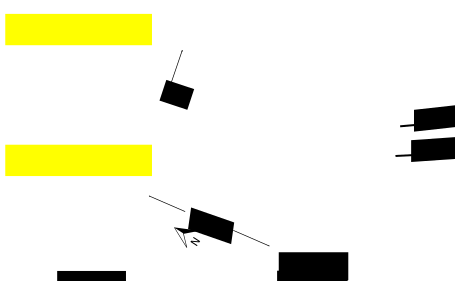
\includegraphics[width=1\linewidth]{altos_reconstructions.pdf}
\end{center}
   \vspace{-0.6cm}
   \caption{3D altocumulus cloud recovery results. (a,b) Sample frames.
   (c,d)  Cross-sections of the recovered cloud-occupancy field $\{\tilde T_k\}$. Cloud
   altitude is above sea-level.}
\label{fig:alto}
\end{figure}
Accounting for the altitude of STARS, these estimated clouds mainly reside on a horizontal layer at $\approx 3450\pm500$m above sea-level. Here, the radiosonde indicated a layer of high humidity that can yield clouds in height range $[3072,4180]$m above sea-level. This is in strong agreement with our results.



%%%%%%%%%%%%%%%%%%%%%%%%%%%%%%%%%%%%%%%%%%%%%%%%%%%%%%%%%%%%%%
\section{Discussion}
\label{sec:discuss}

Scaling light-field imaging hugely to sense the sky, would use  a large network of camera nodes, each having a wide field of view, deployed over a wide area. Such a network can reach anywhere communication exists. This sensing approach offers significant advantages over existing technologies (experimental and operational) of atmospheric sensing, particularly  3D imaging, and doing so in high spatio-temporal resolution. This sensing approach poses new questions for computer vision and computational photography. These include network-based extensions to monocular tasks including network-based radiometric calibration and background estimation. Network redundancy offers the ability of by-passing saturation or blind spots, as those created by the sun, without moving parts.

To enable a massive network, each node should have very low-cost. To demonstrate this can work, units in the small STARS used very basic components and coarse alignment. This concept can spawn more interesting research. In the direction of the sun blocker, other sensors can be incorporated. Night-time operation is an interesting challenge. Furthermore, such a light-field system can be used for studying airborne animals (birds, bats~\cite{bats2010}, locust), in 3D time-lapses.


%%%%%%%%%%%%%%%%%%%%%%%%%%%%%%%%%%%%%%%%%%%%%%%%%%%%%%%%%%%%%%
\section{Acknowledgments}
\label{sec:acknow}
We are grateful to Pinhas Alpert, Daniel Rosenfeld, Orit Altaratz-Stollar, Nir Stav, Raanan Fattal, Arnon Karnieli, David Diner and Anthony Davis for useful discussions and Amit Savir for directing us to radiosonde data. We thank Mark Shenin and Technion building superintendents for experiment assistance. We thank Johanan Erez, Ina Talmon, Tamar Galateanu and Dani Yagodin for technical support. Yoav Schechner is a Lanadu Fellow - supported by the Taub Foundation. His research is supported in part by the Israel Science Foundation (ISF Grant 1467/12) and the Asher Space Research Institute. This work was conducted in the Ollendorff Minerva Center. Minerva is funded through the BMBF.




%===========================================================
\bibliographystyle{splncs}
%\bibliography{cloudsbib}
\begin{thebibliography}{10}

\bibitem{Adelson1992}
Adelson, E., Wang, J.:
\newblock {Single lens stereo with a plenoptic camera}.
\newblock IEEE Trans. PAMI \textbf{14} (1992)  99--106

\bibitem{Basha2012}
Basha, T., Avidan, S., Hornung, a., Matusik, W.:
\newblock {Structure and motion from scene registration}.
\newblock Proc. IEEE CVPR (2012)  1426--1433

\bibitem{bishop}
Bishop, T.E., Zanetti, S., Favaro, P.:
\newblock {Light field superresolution}.
\newblock Proc. IEEE ICCP \textbf{129} (2009)  1--9

\bibitem{horstmeyer}
Horstmeyer, R., Euliss, G., Athale, R., Levoy, M.:
\newblock {Flexible multimodal camera using a light field architecture}.
\newblock In: Proc. IEEE ICCP  (2009)  1--8

\bibitem{Ng1948}
Levoy, M., Ng, R., Adams, A., Footer, M., Horowitz, M.:
\newblock {Light field microscopy}.
\newblock ACM TOG \textbf{25} (2006)  924----934

\bibitem{kim}
Kim, J., Lanman, D., Mukaigawa, Y., Raskar, R.:
\newblock {Descattering transmission via angular filtering}.
\newblock In: Proc. ECCV  (2010)  86--99

\bibitem{Stelamaris2014}
Alterman, M., Swirski, Y., Schechner, Y.Y.:
\newblock {STELLA MARIS}: Stellar marine refractive imaging sensor.
\newblock In: Proc. IEEE ICCP  (2014)  1--10

\bibitem{diner}
Diner, D.J., Martonchik, J.V.:
\newblock {Atmospheric transmittance from spacecraft using multiple view angle
  imagery}.
\newblock Appl. Opt. \textbf{24} (1985)  3503--3511

\bibitem{Diner1998}
Diner, D.J., Beckert, J.C., Reilly, T.H., Bruegge, C.J., Conel, J.E., Kahn,
  R.A., Martonchik, J.V., Ackerman, T.P., Davies, R., Gerstl, S.A.:
\newblock {Multi-angle imaging spectro-radiometer (MISR) instrument description
  and experiment overview}.
\newblock IEEE Trans. Geoscience and Remote Sens. \textbf{36} (1998)
  1072--1087

\bibitem{dinerDavis07}
Diner, D.J., Davis, A., Hancock, B., Gutt, G., Chipman, R.A., Cairns, B.:
\newblock {Dual-photoelastic-modulator-based polarimetric imaging remote
  sensing}.
\newblock Appl. Opt. \textbf{46} (2007)  8428--8445

\bibitem{dinerDavis10}
Diner, D.J., Davis, A., Hancock, B., Geier, S., Rheingans, B., Jovanovic, V.,
  Bull, M., Rider, D.M., Chipman, R.A., Mahler, A.B., McClain, S.C.:
\newblock {First results from a dual photoelastic-modulator-based polarimetric
  camera}.
\newblock Appl. Opt. \textbf{49} (2010)  2929

\bibitem{baxter}
Baxter, B., Hooper, B.A., Williams, J.Z., Dugan, J.P.:
\newblock {Polarimetric remote sensing of ocean waves}.
\newblock In: Proc. MTS/IEEE OCEANS  (2009)  1--5

\bibitem{breon}
Brdon, E.M., Br\'{e}on, F.M.:
\newblock {An analytical model for the cloud-free atmosphere/ocean system
  reflectance}.
\newblock Remote Sensing of Environment \textbf{43} (1993)  179--192

\bibitem{vanMol}
Mol, B.V., Ruddick, K., van Mol, B., K.Ruddick:
\newblock {The compact high resolution imaging spectrometer (CHRIS): the future
  of hyperspectral satellite sensors. Imagery of Oostende coastal and inland
  waters}.
\newblock In: Proc. Airborne Imaging Spectroscopy Workshop  (2004)

\bibitem{5753124}
Schechner, Y.Y., Diner, D., Martonchik, J.:
\newblock Spaceborne underwater imaging.
\newblock In: Proc. IEEE ICCP  (2011)  1--8

\bibitem{Aides:13}
Aides, A., Schechner, Y.Y., Holodovsky, V., Garay, M.J., Davis, A.B.:
\newblock {Multi sky-view 3D aerosol distribution recovery}.
\newblock Opt. Express \textbf{21} (2013)  25820--25833

\bibitem{Tomography2014}
Alterman, M., Schechner, Y.Y., Vo, M., Narasimhan, S.G.:
\newblock Passive tomography of turbulence strength.
\newblock In: Proc. ECCV 
\newblock (2014)  47--60

\bibitem{Peng2014}
Peng, Z., Yoo, S., Yu, D., Huang, D., Kalb, P., Heiser, J.:
\newblock {3D cloud detection and tracking for solar forecast using multiple
  sky imagers}.
\newblock In: Proc. ACM Sympos. Applied Computing (2014)  512--517

\bibitem{LitvinovCVPR05}
Litvinov, A., Schechner, Y.Y.:
\newblock {Addressing radiometric nonidealities: a unified framework}.
\newblock In: Proc. IEEE CVPR  (2005)  52--59 vol. 2

\bibitem{Kang2000}
Kang, S., Weiss, R.:
\newblock {Can we calibrate a camera using an image of a flat, textureless
  Lambertian surface?}
\newblock Proc. ECCV (2000)  640--653

\bibitem{Koreban2009}
Koreban, F., Schechner, Y.Y.:
\newblock {Geometry by deflaring}.
\newblock Proc. IEEE ICCP (2009)  1--8

\bibitem{Raskar2008}
Raskar, R., Agrawal, A., Wilson, C.a., Veeraraghavan, A.:
\newblock {Glare aware photography}.
\newblock ACM TOG \textbf{27} (2008)  56:1--56:10

\bibitem{Talvala2007}
Talvala, E.V., Adams, A., Horowitz, M., Levoy, M.:
\newblock Veiling glare in high dynamic range imaging.
\newblock ACM TOG \textbf{26} (2007)

\bibitem{Rouf2011}
Rouf, M., Mantiuk, R., Heidrich, W., Trentacoste, M., Lau, C.:
\newblock {Glare encoding of high dynamic range images}.
\newblock Proc IEEE CVPR (2011)  289--296

\bibitem{Pust2008}
Pust, N.J., Shaw, J.A.:
\newblock Digital all-sky polarization imaging of partly cloudy skies.
\newblock Appl. Opt. \textbf{47} (2008)  H190--H198

\bibitem{bradley}
Bradley, E.S., Toomey, M.P., Still, C.J., Roberts, D.A.:
\newblock {Multi-scale sensor fusion with an online application: Integrating
  GOES, MODIS, and webcam imagery for environmental monitoring}.
\newblock IEEE Selected Topics in Applied Earth Obs. and Remote Sen. \textbf{3}
  (2010)  497--506

\bibitem{jacobs14cloudmap}
Jacobs, N., King, J., Bowers, D., Souvenir, R.:
\newblock {Estimating cloud maps from outdoor image sequences}.
\newblock In: Proc. IEEE WACV (2014)

\bibitem{allmen}
Allmen, M.C., {Kegelmeyer Jr.}, P.:
\newblock {The computation of cloud base height from paired whole-sky imaging
  cameras}.
\newblock Machine Vision and Applications \textbf{9} (1997)  160--165

\bibitem{angeo-27-953-2009}
Baumgarten, G., Fiedler, J., Fricke, K.H., Gerding, M., Hervig, M., Hoffmann,
  P., M\"{u}ller, N., Pautet, P.D., Rapp, M., Robert, C., Rusch, D., von
  Savigny, C., Singer, W.:
\newblock {The noctilucent cloud (NLC) display during the ECOMA/MASS sounding
  rocket flights on 3 August 2007: morphology on global to local scales}.
\newblock Annales Geophysicae \textbf{27} (2009)  953--965

\bibitem{cazorla}
Cazorla, a., Olmo, F.J., Aladosarboledas, L., Alados-Arboledas, L.:
\newblock {Using a sky imager for aerosol characterization}.
\newblock Atmospheric Environment \textbf{42} (2008)  2739--2745

\bibitem{long}
Long, C.N., Sabburg, J.M., Calbo, J., Pages, D., Calb\'{o}, J., Pag\`{e}s, D.:
\newblock {Retrieving cloud characteristics from ground-based daytime color
  all-sky images}.
\newblock J. Atmospheric and Oceanic Technology \textbf{23} (2006)
  633--652

\bibitem{Seiz}
Seiz, G., Shields, J., Feister, U., Baltsavias, E.P., Gruen, A.:
\newblock {Cloud mapping with ground-based photogrammetric cameras}.
\newblock Int. J. Remote Sens. \textbf{28} (2007)  2001--2032

\bibitem{kassianov}
Kassianov, E., Long, C., Christy, J.:
\newblock {Cloud-base-height estimation from paired ground-based hemispherical
  observations}.
\newblock J. Applied Meteorology \textbf{44} (2005)  1221--1233

\bibitem{Seiz2006}
Seiz, G., Davies, R.:
\newblock {Reconstruction of cloud geometry from multi-view satellite images}.
\newblock Remote Sensing of Environment \textbf{100} (2006)  143--149

\bibitem{6528314}
Alterman, M., Schechner, Y.Y., Swirski, Y.:
\newblock Triangulation in random refractive distortions.
\newblock In: Proc. IEEE ICCP  (2013)  1--10

\bibitem{lensky2006time}
Lensky, I., Rosenfeld, D.:
\newblock The time-space exchangeability of satellite retrieved relations
  between cloud top temperature and particle effective radius.
\newblock Atmospheric Chemistry and Physics \textbf{6} (2006)  2887--2894

\bibitem{Mesoscale}
Atkinson, B.W.:
{\em Meso-Scale Atmospheric Circulations}
\newblock Academic Press (1989), 19

\bibitem{Seiz2002}
Seiz, G., Baltsavias, E., Gruen, A.A.:
\newblock {Cloud mapping from the ground: Use of photogrammetric methods}.
\newblock Photogrammetric Eng. and Remote Sensing \textbf{68} (2002)  941--951

\bibitem{lalonde}
Lalonde, J.F., Narasimhan, S., Efros, A.:
\newblock What do the sun and the sky tell us about the camera?
\newblock IJCV \textbf{88} (2010)  24--51

\bibitem{NAV:6418444}
Bennett, G.G.:
\newblock The calculation of astronomical refraction in marine navigation.
\newblock The Journal of Navigation \textbf{35} (1982)  255--259

\bibitem{download}
Clouds in the Cloud webpage and data link\\
\url{http://webee.technion.ac.il/~yoav/research/clouds_inthe_cloud.html}


\bibitem{hosek2012analytic}
Hosek, L., Wilkie, A.:
\newblock An analytic model for full spectral sky-dome radiance.
\newblock ACM TOG \textbf{31} (2012)  95:1--95:9

\bibitem{Kutulakos2000}
Kutulakos, K., Seitz, S.:
\newblock {A theory of shape by space carving}.
\newblock IJCV \textbf{38} (2000)  199--218

\bibitem{Ihrke2004}
Ihrke, I., Magnor, M.:
\newblock Image-based tomographic reconstruction of flames.
\newblock In: Proc. ACM SIGGRAPH  (2004)  365--373

\bibitem{lowe2004distinctive}
Lowe, D.G.:
\newblock Distinctive image features from scale-invariant keypoints.
\newblock IJCV \textbf{60} (2004)  91--110

\bibitem{Supp2014}
Veikherman, D., Aides, A., Schechner, Y.Y., Levis, A.:
\newblock {Clouds in the cloud: supplementary material} 
\newblock for Proc. ACCV (2014)

\bibitem{Yamashita2004}
Yamashita, M.:
\newblock {Cloud cover estimation using multitemporal hemisphere imageries}.
\newblock In: Proc. XXth Congress of the Society for Photogrammetry and Remote
  Sensing  (2004)  818----821

\bibitem{Evans1998}
Evans, K.F.:
\newblock {The spherical harmonics discrete ordinate method for
  three-dimensional atmospheric radiative transfer}.
\newblock Journal of the Atmospheric Sciences \textbf{55} (1998)  429--446

\bibitem{Levoy1990}
Levoy, M.:
\newblock {Efficient ray tracing of volume data}.
\newblock ACM TOG \textbf{9} (1990)  245--261

\bibitem{bats2010}
Breslav, M., Fuller, N., Sclaroff, S., Betke, M.:
\newblock {3D Pose estimation of bats in the wild}.
\newblock In: Proc. IEEE WACV  (2014)

\end{thebibliography}




%this would normally be the end of your paper, but you may also have an appendix
%within the given limit of number of pages
\end{document}
